\documentclass[a4paper, 12pt, titlepage, twoside]{article}

\usepackage[T2A]{fontenc}
\usepackage[utf8x]{inputenc}
\usepackage[russian,english]{babel}
\usepackage{graphicx}
\usepackage{svg}
\usepackage{amsmath} % Для красивых дробей

\usepackage{listings}
\lstset{
  basicstyle=\footnotesize,
  language=Lisp,
  breaklines=true
}

\usepackage{hyperref}
\hypersetup{
    colorlinks=false,
    pdfborder={0 0 0},
}

\usepackage{fullpage}

\begin{document}
\title{How to Structure a LaTeX Document}
\begin{titlepage}
  \begin{center}
    \vspace{10pt}
    \includesvg[height=120pt]{lambda}
    \\
    \vspace{120pt}
    \Huge{Методическое пособие по языку Common Lisp.}
    \end{center}
\end{titlepage}

\section{Lispbox}
Lispbox --- небольшая, но функциональная среда разработки для языка Common Lisp. Она представляет собой текстовый редактор Emacs связанный с лисп-системой Clozure Common Lisp через расширение Slime (\textbf{S}uperior \textbf{L}isp \textbf{I}nteraction \textbf{M}ode for \textbf{E}macs). Также в lispbox входит настроенная для работы система управления пакетами quicklisp. Из-за почтенного возраста ключевого компонента системы --- редактора Emacs, которому в следующем году исполнится 38 лет, некоторые особенности управления могут оказаться странными или запутывающими, однако на практике они оказываются довольно удобными и впоследствии вызывают сильное привыкание.
\subsection{Установка}
Домашняя страница проекта: \url{http://common-lisp.net/project/lispbox/}. Lispbox распространяется в виде zip-архива и не требует установки. Просто скачайте архив и распакуйте его в удобное вам место, например C:\textbackslash{}Users
\textbackslash{}Alex\textbackslash{}Lisp\textbackslash{}lispbox. К сожалению, у lispbox иногда возникают проблемы с кириллическими путями, поэтому может понадобиться распаковка в место, путь к которому содержит только латинские символы.
По-умолчанию lispbox не поддерживает нелатинские символы, но их поддержку несложно добавить. Для это нужно выполнить следующие действия:
\begin{itemize}
\item В директории, в которую вы распаковали lispbox, найдите файл lispbox.bat и замените в нем строку 
\end{itemize} % OMG TEH HAXZ!

\footnotesize
\begin{verbatim}
set TO_EVAL="(progn (load \"lispbox\") (slime))"
\end{verbatim}
\normalsize

\begin{itemize}
\item[] на строку
\end{itemize}

\footnotesize
\begin{verbatim} 
set TO_EVAL="(progn (setq slime-net-coding-system 'utf-8-unix)(load \"lispbox\") (slime))"
\end{verbatim}
\normalsize

\begin{itemize}
\item В подкаталоге slime-* в файле swank-loader.lisp в самое начало файла добавьте строку
\end{itemize}
\footnotesize
\begin{verbatim} 
(setf CCL:*DEFAULT-EXTERNAL-FORMAT* :utf-8)
\end{verbatim}
\normalsize

Теперь lispbox поддерживает русский язык (а также все остальные языки с нелатинской письменностью).

Для запуска среды дважды щелкните по файлу \verb|lispbox.bat|. Если всё прошло успешно, сначала вы увидите лог процесса запуска системы, а потом вас поприветствует следующее окно:
\begin{center}
  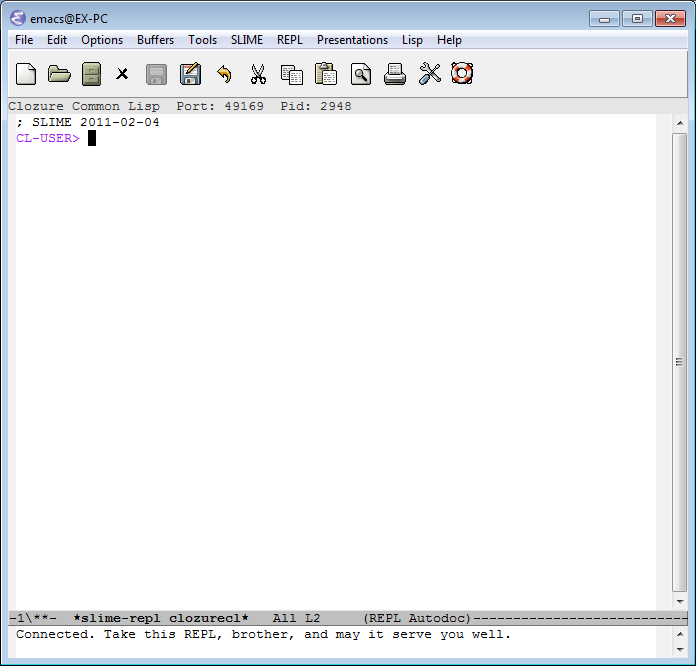
\includegraphics[scale=.6]{lispbox_started}\\
  \small{\textit{Запущенный lispbox}}
\end{center}
\subsection{Работа в lispbox}
Lispbox, как и любая приличная IDE для Лиспа, обладает тремя облегчающими жизнь опциями:
\begin{itemize}
\item ведет подсчет открывающих и закрывающих скобок --- при постановке закрывающей скобки подсвечивается соответсвтующая открывающая
\item автоматически выравнивает исходный код (по нажатию клавиши Tab) как в режиме интерпретатора, так и в режиме редактирования исходного кода
\item подсвечивает исходный код
\end{itemize}
Помимо перечисленного выше, у lispbox есть еще множество особенностей, со многими из которых мы познакомимся позднее.

Emacs --- основа выбранной нами IDE --- крайне гибкий и мощный инструмент, однако, довольно требовательный к пользователю. Безграничный потенциал Emacs и его отличия от традиционных текстовых редакторов породили множество легенд о сложности в освоении и использовании. Но это совсем не так. Совершим небольшой экскурс по основным понятиям и командам Emacs.
\subsubsection{Буфер}
\textit{Буфером} называется во-первых любой открытый файл, а во-вторых вообще любое пространство, в которое вводится или выводится информация. Название буфера пишется внизу слева. Все буферы перечислены в верхнем меню Buffer. Как видно, после старта lispbox по умолчанию открыты буферы под названиями \verb|*scratch*|, \verb|*Messages*|, \verb|*slime-events*|, \verb|*slime-repl clozurecl*| и \verb|*inferior-lisp*|. Первые два являются стандартными буферами Emacs, следующие два --- служебные буферы Slime, и наконец последний --- интерпретатор, открытый сейчас перед нами. Обратите внимание на название буфера, написанное слева внизу.
\begin{center}
  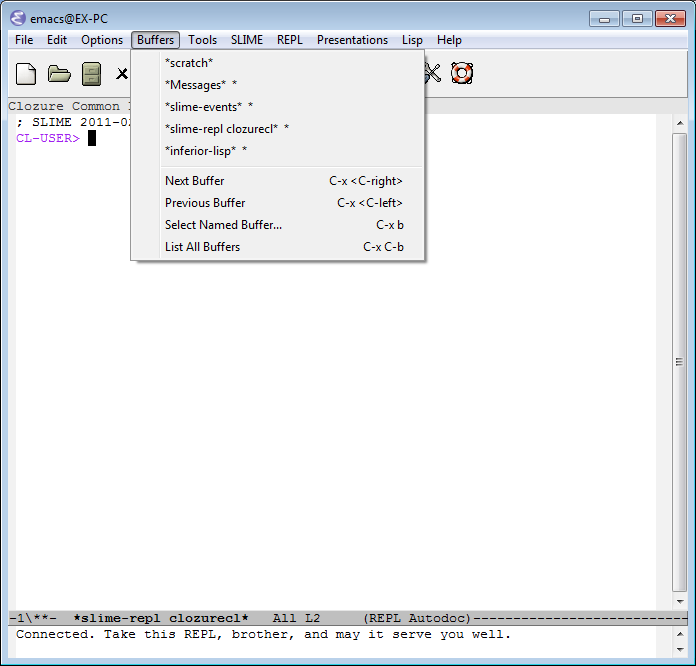
\includegraphics[scale=.6]{lispbox_buffers}\\
  \small{\textit{Буферы по умолчанию}}
\end{center}
\subsubsection{Горячие клавиши}
На рисунке выше внизу выпадающего меню рядом с командами находятся сочетания клавиш, также иногда называемые аккрдами, назначенные на эти команды.
Такие сочетания используются в Emacs повсеместно, и после некоторого привыкания очень сильно облегчают работу. Однако, конвенция, принятая в Emacs, довольно сильно отличается от всех остальны программ, и требует пояснения.

Рассмотрим, к примеру, команду Next-buffer. Как видно из скиншота выше, этой команде назначено сочетание C-x <C-left>. Буквой С в Emacs обозначается нажатие на клавишу Control. Запись C-x обозначает всего-навсего сочетание Control-x. Последовательность C-x <C-left> же означает, что сначала нужно набрать Control-x, а потом Control-<стрелка влево>. Сделать это можно и не отпуская клавишу Control, то есть зажать Control, потом нажать и отпустить x, а потом нажать стрелку влево.
Если префикс С- не указан, значит нажатие на Control не нужно. То есть С-х b есть комбинация Control-x, за которой следует нажатие на кнопку b уже при отпущенной клавише Control. Также существуют сочетания с клавишей Alt, которые записываются как M- (от названия клавиши Meta, отсутствующей на современных клавиатурах).
Основные команды работы с буферами, многие из которых также доступны через меню ``File'' и ``Buffers'', перечислены ниже:
\begin{itemize}
\item C-x C-f открывает файл с с введенным именем. Если файл есть, открывает для редактированияб если нет --- создает новый
\item C-x b <имя буфера> переключается на буфер с введенным именем. Если такого буфера нет, то он будет создан
\item C-x C-b создает новое \textit{окно}, в которое выводит список существует буферов
\item C-x k закрывает буфер, в котором находится курсор. Если буфер остался один, закрыть его нельзя. Если вы попытаетесь закрыть буфер, открытый на файле, и имеющий несохраненные данные, Emacs попросит подтверждения выполнения
\item C-x C-s сохраняет содержимое буфера в текстовый файл
\end{itemize}
\subsubsection{Окна}
Emacs использует термин ``окно'' в несколько отличном от привычного смысле. Окно в том же смысле, в котором его используем мы, то есть в смысле отдельного окна опрерационной системы, в Emacs называется \textit{фреймом}. Окном же называется область, в которой отображается ровно один буфер. Новые окна можно получить, деля существующие по горизонтали или по вертикали. Две команды для работы с окнами можно найти в меню ``File''. Некоторые команды для работы с окнами:
\begin{itemize}
\item C-x 2 делит окно по горизонтали
\item C-x 3 делит окно по вертикали
\item C-x 0 закрывает окно, в котором находится курсор, сливая его с ближайшим соседним окном. Как и в случае с буфером, закрыть последнее открытое окно нельзя. Обратите внимание, что буфер, отображавшийся в окне, никуда не пропадает, и вернуться к нему можно при помощи команды C-x b
\item C-x 1 разворачивает выбранное окно на весь фрейм. Также это можно трактовать как закрытие всех окон, кроме выбранного
\end{itemize}
\subsubsection{Работа с текстом}
\begin{itemize}
\item <C-space> начинает выделение текста, аналогично обычному выделению мышью
\item C-w вырезать
\item M-w копировать
\item C-y вставить
\item C-/ аналог Ctrl-z
\item C-p, C-n перейти на предыдущую/следующую строку (стрелки вверх и вниз)
\item C-f, C-b перейти на символ вперед/назад (стрелки вправо и влево)
\item C-a, C-e перейти в начало/конец строки (клавиши Home и End)
\item M-f, M-b
\item M-d
\item <M-backspace>
\end{itemize}
\subsection{Интерпретатор}
Итак, среда запущена и готова к работе. Вы видите перед собой приглашение, гласящее \verb|Cl-USER>|. Такой режим работы Лиспа называется REPL --- Read-Eval-Print Loop, также известный как интерактивный режим или \textit{toplevel}. Суть его заключается в том, что пользователь напрямую общается с лисп-системой, производя вычисления и получая ответы в реальном времени. Этот режим, впервые появившийся в Лиспе, отличает его от статических, компилируемых языков типа Фортрана, С или Java, и присутствует практически во всех динамических языках, например Ruby, Python и Perl. Несмотря на то, что этот режим присущ интерпретируемым языкам, почти все современные реализации Common Lisp являются компилируемыми, и Clozure CL в этом плане не исключение.

Числа и строки являются самыми простыми выражениями, доступными программисту, и вычисляются сами в себя. Поприветствуйте lispbox, введя в строке приглашения что-нибудь вроде ``Привет, Лисп!'', и нажав Enter. Строка, введенная вами, выведется на экран, а после неё снова появится строка приглашения. То же самое произойдет, если вводить числа, простые и десятичные дроби, а также некоторые другие выражения:
\begin{center}
  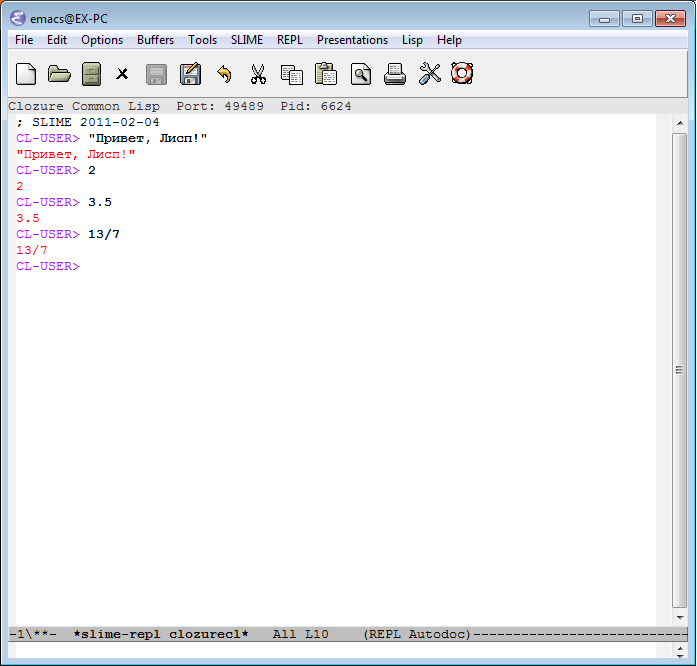
\includegraphics[scale=.7]{lispbox_toplevel}\\
  \small{\textit{Простейшие выражения}}
\end{center}
Теперь рассмотрим некоторые более сложные примеры команд. Например, если мы хотим сложить два числа 1 и 2, следует ввести \verb|(+ 1 2)|. Как несложно заметить, такая запись несколько отличается от принятой и в математике, и в других языках программирования. Это непривычно, однако более универсально: для записи сложения трех чисел обычная запись требует использования уже двух знаков ``+'', в то время как в префиксной нотации, принятой в Лиспе, сложение трех чисел будет выглядеть так: \verb|(+ 1 2 3)|. Таким образом, операция сложения может принимать произвольное количество агрументов, а может и не принимать ни одного арумента вообще. Умножение работает точно таким же образом. Вычитание и деление отличаются тем, что должны принимать хотя бы один агрумент --- соответственно, уменьшаемое и делимое.

Выражения могут быть вложенными: \verb|(+ (* 2 3 4) (/ 10 3))|. Так как количество агрументов может быть произвольным, скобки служат для обозначения границ выражений. Выражения Лиспа также называются \textit{формами}. В дальнейшем будем считать эти термины синонимами. % А на самом деле они синонимичны?
Большие формы с глубокой вложенностью удобно записывать, разбивая на несколько строк, каждую из которых можно выровнять нажатием на клавишу Tab.

Числовые значения, как и строки, представляют собой так называемые \textit{атомы}. В Лиспе возможны всего два типа выражений --- атомы и списки, причем сам код программы тоже является списком. Это одно из важнейших свойств Лиспа, из которого вытекает множество интересных последствий, и благодаря которому Лисп заслужил звание программируемого языка программирования.
\begin{center}
  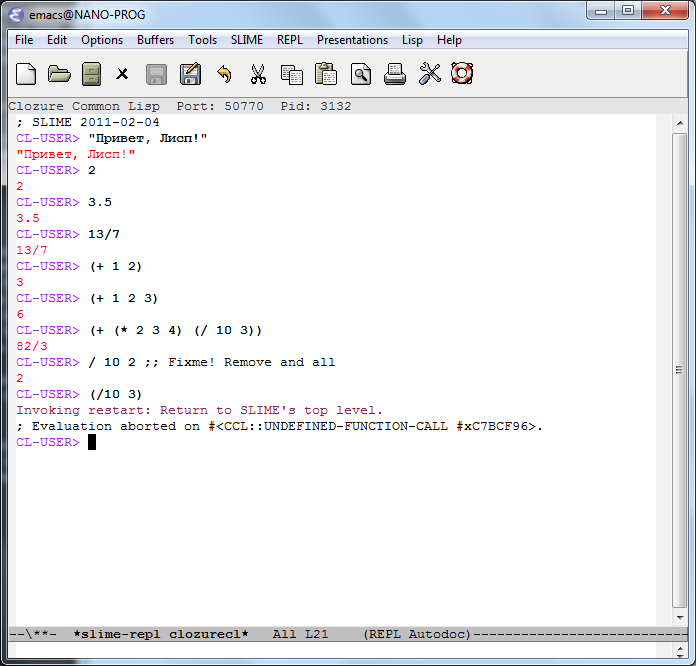
\includegraphics[scale=.7]{lispbox_more_complex}\\ %Тут обязательно надо что-то со вложенностью и примером выравнивания форм
  \small{\textit{Более сложные формы}}
\end{center}
\subsubsection{Ошибки}
Если вы допустите какую-либо ошибку, lispbox остановит выполнение вычисления и сообщит вам о найденном несоотвествии. Помимо вывода информации о том, что за ошибка произошла, и чему в этот момент были равны значения переменных, lispbox поинтересуется, что делать дальше. В подавляющем большинстве вариантов нас будет интересовать вариант \verb|[*ABORT]|, возвращающий нас к строке приглашения. Он будет перечислен в списке вариантов под определённым номером, но удобнее воспользоваться горячей клавишей q, нажатие на которую вернёт нас из списка возможных рестартов в интерпретатор.
\begin{center}
  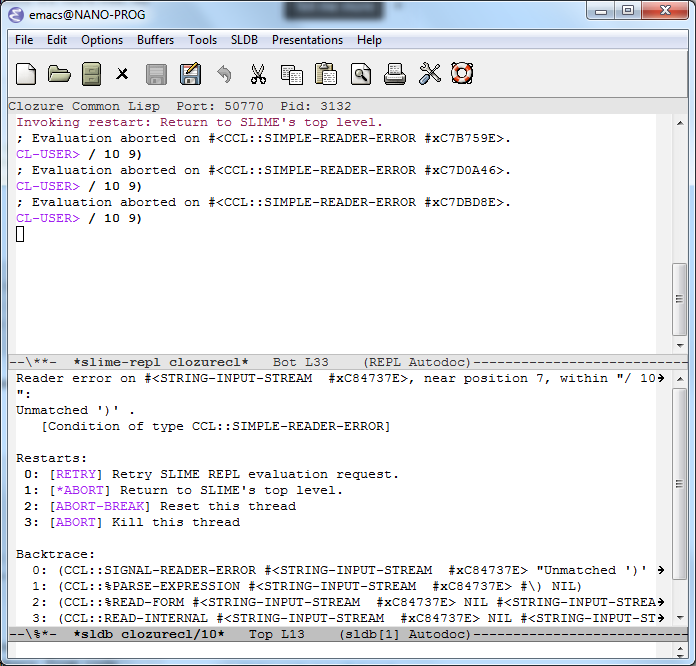
\includegraphics[scale=.7]{lispbox_error_conditions}\\
  \small{\textit{Сообщение об ошибке и список\\возможных вариантов развития событий}}
\end{center}
\subsubsection{Задание 1}
Запишите на Лиспе следующее арифметическое выражение:\\
\[
\cfrac{((24 - 12) + (6 - 3))\cdot\cfrac{6.9 - 3.2}{((4 - 1)\cdot(4 + 1)\cdot(4 - 5))}}{13 - 5}
\]
\newpage
\section{Основы Лиспа}
В этом разделе будут подробно рассмотрены общие для всех диалектов выразительные средства, неизменные с 1956-го года и присутствующие в любом диалекте Лиспа, существующем в наши дни, в том числе и в Common Lisp.
\subsection{Типы данных}
Все типы данных, с которыми может работать Лисп, можно разделить на две глобальные группы --- простые и составные. Простые типы данных, также называемые атомарными, с свою очередь делятся на числовые и символьные. Значение считается числовым, если начинается с цифры, знаков \verb|+|  или \verb|-|, и записано в обычной для чисел форме. Все остальные значения являются символьными. В записи символа можно использовать буквы, цифры, и спецсимволы, но есть пара ограничений: символы не могут начинаться со знака \verb|#|. С этого знака начинаются \textit{макросы чтения}, используемые в том числе для записи составных данных. Они будут рассмотрены позднее. % Или не будут
Также в названиях символов нельзя использовать знаки \verb|( ) ' ` ,|. Регистр букв в записи не имеет значения. То есть \verb|eyem-the-strongest| и \verb|eyem-the-STRONGEST| --- две разные записи одного и того же символа.

Примеры числовых значений:
\begin{itemize}
\item 10
\item -23.5
\item +44/13
\end{itemize}
Примеры символьных значений:
\begin{itemize}
\item x
\item kitty-cat
\item +$-$10
\item +43/$-$32
\item cack315\#1ie!
% \item Сюда обязательно вставить table flip!
\end{itemize}

\end{document}
        

